	Although there are many factors such as diversity, coverage, serendipity that determine the efficiency of recommendation systems, in this project we focused on accuracy and decided to leave other factors outside the scope of this project.
	\subsubsection{Methods}
	\paragraph{Leave-one-out Cross Validation} \mbox{} \\
	In Leave-one-out Cross Validation, for the dataset with n data in the original sample then, n-1 samples are used as training set while the remaining data is used to test accuracy. This process is repeated for all n data and the final result calculated by taking the average of these n tests.
	
	\paragraph{Shuffle Split Cross Validation} \mbox{} \\
	 \href{https://surprise.readthedocs.io/en/stable/model_selection.html#surprise.model_selection.split.ShuffleSplit}{Shuffle Split Cross Validation} randomly samples the dataset during each iteration to generate training and test sets. For the Shuffle Split CV, number of splits was chosen as 3 and the final result calculated by taking the average of these three iterations.
	
	\subsubsection{Results}
	\paragraph{Stockmount} \mbox{}\\
	\textbf{About the dataset:} Dataset origanally consists of 142501 customers and 73482 products with implicit ratings (i.e. purchased or not). However, to make the customer versus product matrix a little denser, customers with less than 2 products and products with less than 2 customers are eliminated. After filtering,
	\begin{center}
		\begin{tabular}{ | c | c |}
			\hline
			& filtering threshold = 2\\ 
			\hline
			Number of Customers & 2182\\  
			\hline
			Number of Products & 1355\\  
			\hline
			Number of Communities & 175\\  
			\hline
			Sparsity & 99.808124 \% \\   
			\hline
		\end{tabular}
	\end{center} 
	\vspace{0.5cm}
	\textbf{Testing method:} Since the dataset contains implicit ratings, I preferred to use "Hit Rate" rather than RMSE or MAE as the test metric and "Leave-one-out CV" as the cross validation iterator. Basically, for each deleted transaction, test module checked whether the product in the deleted transaction was within the recommended products.\\
	\textbf{Tested Recommender:} Eigentrust Weighted Trust Based Recommender \ref{eigentrust_section} \\ \\
	\textbf{Results:}
	\begin{center}
		\begin{tabular}{ | c | c | c |}
			\hline
			& 5 Recommendations & 10 Recommendations\\ 
			\hline
			Number of Tests&  4160 & 4160\\  
			\hline
			Number of Hits&  1367 & 1983\\  
			\hline
			Hit Rate &   0.328605 & 0.476682\\  
			\hline
		\end{tabular}
	\end{center} 
	Results were analysed on the basis of community density, community size and number of products purchased by the customer, but no significant correlation with accuracy found.
	
	\paragraph{Amazon Food Reviews \cite{Amazonfoodreviews}} \mbox{}\\
	\textbf{About the dataset:} 
	\begin{center}
		\begin{tabular}{ | c | c |}
			\hline
			&Amazon Food Reviews (threshold = 10)  \\  
			\hline
			Number of Users & 4276 \\
			\hline
			Number of Products & 1140 \\
			\hline
			Rating Range & 1-5 \\
			\hline
		\end{tabular}
	\end{center} 
	\vspace{0.5cm}
	\textbf{Testing method:} For this dataset, I wanted to see how efficiently the recommender works on extremely sparse datasets, as a result I preferred to use "Shuffle Split CV" as the cross validation iterator since it is easy to set up the test and training set ratios. The tests with the test set size greater than 0.5 were applied to see the performance of the implemented recommender in cold start and to understand how it improved the collaborative filtering method using the "mean squared difference similarity". As the test metrics, RMSE and MAE were used. Tests were performed using Surprise.\\
	\textbf{Tested Recommender:} Inverse Distance Weighted Trust Based Recommender (with the Proposed Method 2)\ref{inverse_section} \\ \\
	\textbf{Benchmark:} \\
	\textbf{Test set: 0.2, Training set: 0.8, Sparsity: 0.9891}
	\begin{center}
		\begin{tabular}{ | c | c | c | c | c | c | c | c |}
			\hline
			& Trust Based & MSD & SVD & Slope One & KNN & NMF & CoCluster\\ 
			\hline
			RMSE&0.6727  & 0.6443  & 0.6944  & 0.7167  & 0.6615  & 0.6661  & 0.7199\\
			\hline
			MAE&0.3321  & 0.3089  & 0.471  & 0.4049  & 0.395  & 0.4131  & 0.4441\\
			\hline
		\end{tabular}
	\end{center} 
	\vspace{1cm}
	\textbf{Test set: 0.3, Training set: 0.7, Sparsity: 0.9904}
	\begin{center}
	\begin{tabular}{ | c | c | c | c | c | c | c | c |}
		\hline
		& Trust Based & MSD & SVD & Slope One & KNN & NMF & CoCluster\\ 
		\hline
		RMSE&0.672  & 0.6599  & 0.7252  & 0.7226  & 0.6906  & 0.6852  & 0.7133\\
		\hline
		MAE&0.3375  & 0.3239  & 0.5081  & 0.4074  & 0.4203  & 0.4308  & 0.415\\
		\hline
	\end{tabular}
	\end{center} 
	\vspace{1cm}
	\textbf{Test set: 0.4, Training set: 0.6, Sparsity: 0.9918}
	\begin{center}
	\begin{tabular}{ | c | c | c | c | c | c | c | c |}
		\hline
		& Trust Based & MSD & SVD & Slope One & KNN & NMF & CoCluster\\ 
		\hline
		RMSE&0.7012  & 0.7211  & 0.7633  & 0.7396  & 0.7231  & 0.7086  & 0.7156\\
		\hline
		MAE&0.3636  & 0.3594  & 0.5548  & 0.4146  & 0.4458  & 0.4491  & 0.4232\\
		\hline
	\end{tabular}
	\end{center} 
	\vspace{1cm}
	\textbf{Test set: 0.5, Training set: 0.5, Sparsity: 0.9931}
	\begin{center}
	\begin{tabular}{ | c | c | c | c | c | c | c | c |}
		\hline
		& Trust Based & MSD & SVD & Slope One & KNN & NMF & CoCluster\\ 
		\hline
		RMSE&0.7331  & 0.7784  & 0.8212  & 0.7648  & 0.7562  & 0.7447  & 0.7624\\
		\hline
		MAE&0.3975  & 0.3971  & 0.6144  & 0.429  & 0.4835  & 0.4848  & 0.463\\
		\hline
	\end{tabular}
	\end{center} 
	\vspace{1cm}
	\textbf{Test set: 0.6, Training set: 0.4, Sparsity: 0.9945}
	\begin{center}
	\begin{tabular}{ | c | c | c | c | c | c | c | c |}
		\hline
		& Trust Based & MSD & SVD & Slope One & KNN & NMF & CoCluster\\ 
		\hline
		RMSE&0.7719  & 0.91  & 0.8787  & 0.7879  & 0.8241  & 0.7949  & 0.7545\\
		\hline
		MAE&0.4382  & 0.481  & 0.676  & 0.4437  & 0.5419  & 0.5217  & 0.4422\\
		\hline
	\end{tabular}
	\end{center} 
	\vspace{1cm}
	\textbf{Test set: 0.7, Training set: 0.3, Sparsity: 0.9958}
	\begin{center}
	\begin{tabular}{ | c | c | c | c | c | c | c | c |}
		\hline
		& Trust Based & MSD & SVD & Slope One & KNN & NMF & CoCluster\\ 
		\hline
		RMSE&0.8671  & 1.1469  & 0.9456  & 0.8266  & 0.9157  & 0.863  & 0.8238\\
		\hline
		MAE&0.5186  & 0.6468  & 0.739  & 0.4611  & 0.6179  & 0.5848  & 0.5065\\
		\hline
	\end{tabular}
	\end{center} 
	\vspace{1cm}
	\textbf{Test set: 0.8, Training set: 0.2, Sparsity: 0.9970}
	\begin{center}
	\begin{tabular}{ | c | c | c | c | c | c | c | c |}
		\hline
		& Trust Based & MSD & SVD & Slope One & KNN & NMF & CoCluster\\ 
		\hline
		RMSE&0.9893  & 1.5542  & 1.0201  & 0.9124  & 1.0562  & 0.9721  & 0.877\\
		\hline
		MAE&0.6396  & 0.9878  & 0.8088  & 0.5124  & 0.7207  & 0.7005  & 0.5391\\
		\hline
	\end{tabular}
	\end{center} 
	\vspace{1cm}
	\textbf{Test set: 0.9, Training set: 0.1, Sparsity: 0.9979}
	\begin{center}
	\begin{tabular}{ | c | c | c | c | c | c | c | c |}
		\hline
		& Trust Based & MSD & SVD & Slope One & KNN & NMF & CoCluster\\ 
		\hline
		RMSE&1.2693  & 2.2067  & 1.106  & 1.0236  & 1.2687  & 1.1095  & 1.0273\\
		\hline
		MAE&0.8898  & 1.6609  & 0.8843  & 0.615  & 0.919  & 0.8506  & 0.6876\\
		\hline
	\end{tabular}
	\end{center} 

\begin{figure}[H]
	\centering
	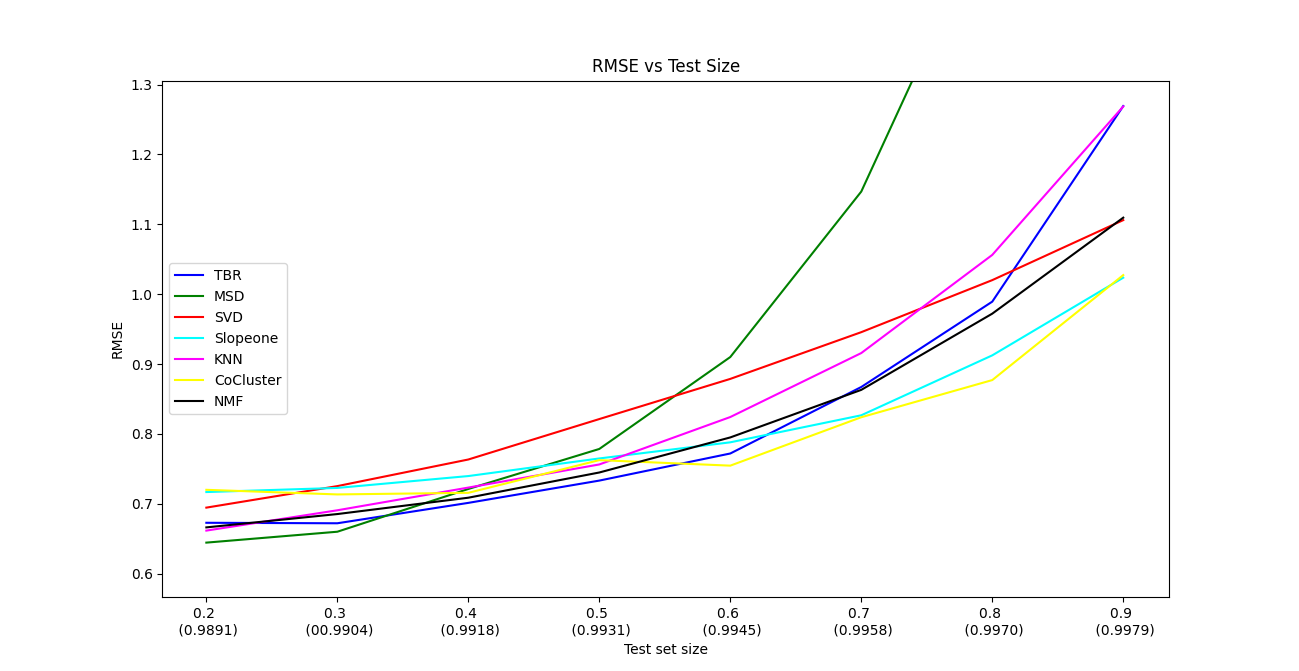
\includegraphics[scale=0.42]{rmse.png}
	\caption{RMSE versus Test set Size. For instance, 0.2 means test set-training set ratio is $20\%-80\%$ . Additionally, floats in parentheses represent the sparsity of training set for corresponding test set size}
	\label{fig:rmse}
\end{figure}

\begin{figure}[H]
	\centering
	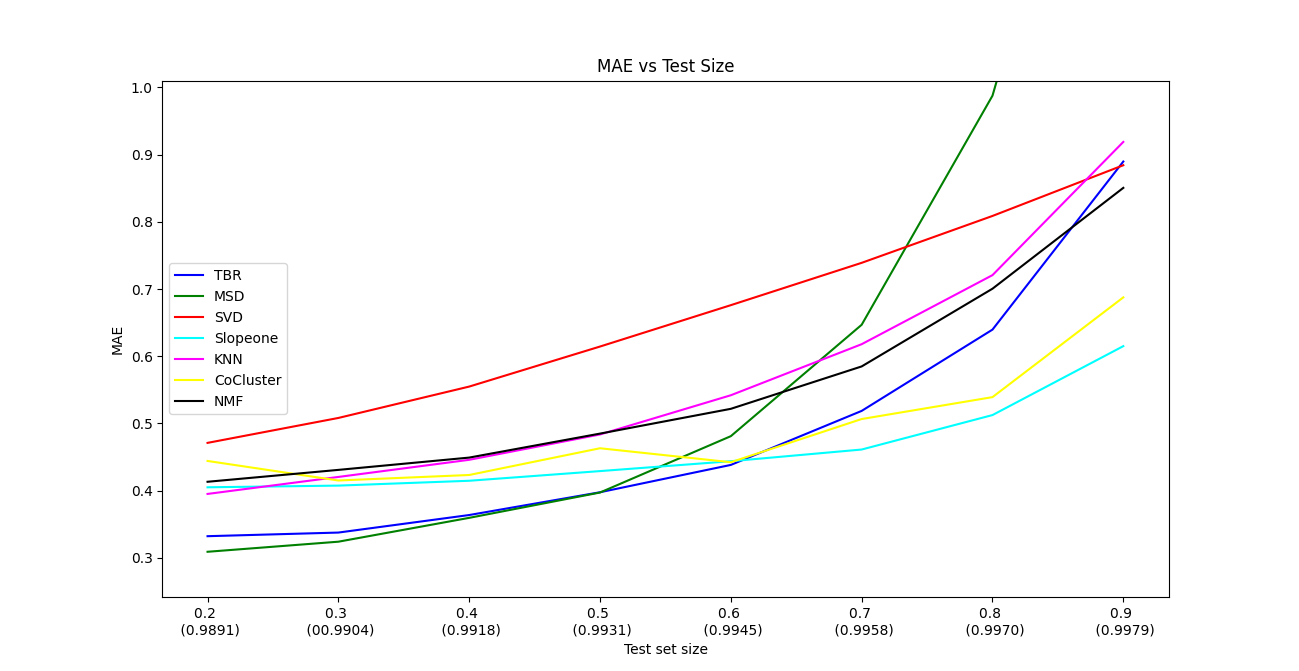
\includegraphics[scale=0.42]{mae.png}
	\caption{MAE versus Testset Size}
	\label{fig:mae}
\end{figure}